\documentclass[hidelinks,english]{article}

\usepackage{graphicx}
\usepackage{grffile}
\usepackage[T1]{fontenc}
\usepackage{babel}
\usepackage{wrapfig}
\usepackage{hyperref}

\date{\today}

\graphicspath{{Pictures/}}
\begin{document}	
	\begin{titlepage}
		\pagenumbering{gobble}
		\begin{figure}[!t]
			
\includegraphics[width=\linewidth]{up_logo.png}
		\end{figure}
		\vspace*{\stretch{1.0}}
		\begin{center}
			\huge{Software Requirements Specification and Technology Neutral Process Design\\}
			\huge{Mindmap PIM}\\
			\large{Client: IMINISYS}\\
			\vspace{10mm}
			\huge{Team: A-Cube-N}\\
		\end{center}
		\begin{center}
			\begin{tabular}{ c c c }
				Dunkley, Nathan & Grobler, Arno & Lochner, Amy \\
				\texttt{14145759} & \texttt{14011396} & \texttt{14038600}\\
				& Maree, Armand &\\
				& \texttt{12017800} &
			\end{tabular}
		\end{center}
		\begin{center}
			Department of Computer Science, University of Pretoria
		\end{center}
		\vspace*{\stretch{2.0}}
	\end{titlepage}
	\newpage
	\tableofcontents
	\newpage
	\pagenumbering{arabic}
	
	\section{Introduction} 
	People of this day and age often make use of many technologies and platforms for the purpose of staying in contact with people, sharing moments with friends, communicating with people and organising their day-to-day lives. Generally all the above tasks of a person in the 21st century are done on different platforms for example Facebook, Email and Google Calendar. This project serves to provide the people described above, with a single PIM platform with which they can interact to make use of the functionality from other platforms. A PIM as defined by \textit{TechTerms} is "a software application that serves as a planner, notebook, and address book all in one. It can also include things like a calculator, clock , and photo album." 
	
	
	\section{Vision}
	The vision of this project is to create an PIM which extracts data from various existing platforms such as Facebook, Gmail, Google Calendar etc. The application will make use of various means to extract data, determine the general topic of the data then either construct a new branch in the mind map or add the data as a sub branch in the diagram. The hope is that this will simplify the users life by only needing one application to 'monitor' all other platforms on which they might have an account and manager the information of those platforms from our application.
	
	\section{Background}
		\subsection{The client's problem}
		
		
		\subsection{Future business/research opportunities}
		
		
	\section{Scope}
	
	
	\section{Software Architecture Overview}
	
	
	\section{Architecture Requirements}
		
		\subsection{Access Channel Requirements}
    		\subsubsection{Human Access Channels}
                Users  will access the "Mind mapped PIM" system through a website. It should be available to anyone wishing to sign up  through any browser i.e. Chrome, Mozilla Firefox, Internet Explorer, Safari and Edge. When on the website, the user will have to log in, the option given to log in with their Facebook or Google user name and passwords.  The website will be under strict standards-compliance that is having the website comply with the World Wide Web Consortium (W3C) (W3C, 2016)  so that the website will run on every browser exactly the same. The website should be mobile friendly as to be able to scale down to a phone screen size and still be usable and interactive. Offline capabilities for users who have already used the service before should also be allowed.
            \subsubsection{System Access Channels}
                RESTful web services will as the system access channel for its lightweightedness, maintainability, and scalability. It will use URI's to allow easy access from the client side web service to server side. 
		
		\subsection{Quality Requirements}
            The following quality requirements have been placed in order of priority.
            \subsubsection{Performance}
                Performance has the highest priority since this system has to be real time. Any new information that is updated on the respective websites and email clients should, in the least amount of time possible, update the mind map too. \\
                
                Performance in terms of front-end should also be addressed. The system is a fully graphic website and thus should give the user the most fluid and smooth experience. To implement a fast interactive system technologies such as SVG or HTML canvas can be used to render the graph with smooth user interaction.
            \subsubsection{Usability}
                Usability is the second highest priority as the system is fully graphic in terms of what the end user will use. The system needs to have a very good UX and must be completely user friendly so it is not difficult to use. The end goal is to let the system give benefit to it being graphic so the user can interpolate the data, and not make it more difficult
            \subsubsection{Reliability}
                The system needs to be reliable, since it has to provide information in real time. this cannot happen if the system is constantly down or can only cater for X amount of users before it starts slowing down. When, for example, a user clicks to expand a bubble the result should be almost instant and not break the graph or slow down the whole system because it is retrieving a few bubbles.\\
                
                Reliability also refers to providing accuracy, and such needs to be implemented to provide the correct information to the right bubbles.
                \\
                Implementation of reliability should be done in two parts, namely first prevention of faults, and secondly detection of faults.
            \subsubsection{Scalability}
                this system needs to be highly scalable both in terms in the non restriction on the amount of users that can use the system simultaneously and the amount of data stored of each user that needs to be both stored and displayed without hindering the rest of the system.\\
            
                
                The amount of users using the system could be large at any time, and the use of the system by one user should not impact the use of the system by another user. The actual Mind map should also not become slower or unresponsive if the amount of bubbles grow, which it will.\\
                
                Polling of the respective social media and email should also be considered. The increase in the amount of threads used for this operation should not make the system unresponsive
            \subsubsection{Flexibility}
                The system must be flexible in terms of plugablity of subsystems that are used namely our social media and emails. Since all of these system are different and use different API's and architectures. The system should be able to handle this, and any future systems that need to be added.\\
                Some users will not have a Facebook account for example, and thus the system should still irrespective if the user has a certain social media.

            \subsubsection{Security}
                The system should be very secure since it is using private information that belongs solely to that user. Private information such as emails and photos isn't something that users would like other people seeing. Thus implementation of a secure log in process has to be implemented. Since Google and Facebook have both good log in systems, we will use that to log in to the system.\\
                If a user prefers to not have certain features of social media, such as only look at posts and photos on Facebook but not post on their behalf, then the system should cater for that.
            \subsubsection{Auditability/Monitorability}
                Logs of all actions and settings of the user should be maintained. When the user logs back in at a different time, the graph that was displayed before should be displayed again and updated with new things that had happened while the user was offline. Settings should remain the same between sessions. Logs will be used to track any unhandled exceptions or problems.
            \subsubsection{Integrability}
                The system should be integrable in terms of how well it integrates with other systems like Facebook and Google. This information should be easy to access and does not affect the functioning of the overall system.

		
		\subsection{Integration Requirements}
		\begin{enumerate}
        \item \textbf{HTTP:}\\
            This is the main protocol for all websites and will be the interface for the user to easily navigate the system.
        \item \textbf{SMTP and IMAP:}\\
            Sometimes a user does not want to connect their social media for safety concerns and so the system cannot use the APIs required and thus will need to manually get the information by making use of IMAP to retrieve and sort though the users mailbox and SMPT to still have the option for the system to send emails on behalf of the user. This allows the system to still have functionality without any specified API's for those users who do not wish to share that information or who do not own social media.\\
        \item \textbf{REST:}\\
            As mentioned before, REST will be implemented. It is simple to implement and integrates well with systems already operational. REST integrates will with HTTP and follows a client-server model which is something our system utilizes. REST is vital to the use of API's to gain access to information of social media of the user.\\
        \item \textbf{TCP:}\\
            This protocol will be needed to establish network connections between the users computers and the system servers. Theses data streams can then be exchanged between the connected hosts. TCP will allow for error detection and rectification of data transmission. This will be done at a high level and would typially be handled by libraries or the OS.\\
        
        \item \textbf{API:}\\
            Since the system will gather its information through the consented use of the users social media, a vital part of the system is to use the already well developed infrastructure created by social media and access the information through API's or application programming interfaces. We will use API's from Google (\sloppy\url{https://developers.google.com/apis-explorer/\#p/}) to access contacts, email, calender, hangouts/sms, Facebooks API (\sloppy\url{https://developers.facebook.com/products}) for Facebook content and LinkedIn API(\sloppy\url{https://developer.linkedin.com/docs/rest-api}) for LinkedIn related information.\\
    \end{enumerate}
		
		\subsection{Architecture Constraints}
			Technical constraints include:
			\begin{itemize}
				\item \textbf{Programming language} We will be developing the system in Java.
				\item \textbf{Operating system} The server will be run off a Linux machine. 
			\end{itemize}
			Further there are no constraints and the architects have free roam to implement an architecture that suits their needs.
			
	\section{Architecture Design}
	
		\subsection{Architectural components addressing architectural responsibilities}
		
		\subsection{Infrastructure}
		
		\subsection{Tactics}
		
	\section{Database and Persistence}
	
	
	\section{Process Specification}
		\subsection{Server}
		In the back end, the system would have a polling service that polls the social media sites for new information about the users. If a polling thread receives new data from the platform they add this new data to a queue to be processed. Several worker threads dequeue data from the queue and uses the natural language processing to determine the topic(s) of the data. This data is then added to a database and the corresponding topic(s) as well. Note that since hashtags are used so frequently, any hashtag in the text should be added as a topic of its own. When a user requests their mind map, the system responds with all relevant topics of their life based on frequency and recency. These topics are then returned to the user in the form of JSON objects. Once a user expands one of the bubbles a request is sent to the server to retrieve all the relevant articles corresponding to the topic to the user. These new data is then added to the mind map in the form of bubbles. Relevant articles are found on the basis of your own events and the events of your friends.
		
		\subsection{Front End}
		The user starts out with a root bubble that has relevant topics connected to it including a friends bubble. All these bubbles can be expanded and reveal information related to that topic. The friends bubble shows contacts you recently communicated with or might want to communicate with now. Expanding one of these contacts will show the different platforms you can interact with this contact, including viewing a profile and sending a message/email. Other topics will expand into relevant articles and those can be expanded again and so forth. Upon expanding an article a user can then interact with that article (comment/reply) in a side panel that will be presented on the right of the screen.
	
	\section{Functional Requirements}		
		\subsection{Use Case Prioritisation}
			\textbf{Critical}
			\begin{itemize}
			    \item Sign up
			    \item Choose your data sources
			    \item Login to Data Sources
			    \item Logout
			    \item Delete Account
			\end{itemize}
			\textbf{Important}
			\begin{itemize}
			    \item Specify the initial depth
			    \item Specify the branch factor
			    \item Specify filter
			\end{itemize}
			\textbf{Nice-to-Have}
			\begin{itemize}
			    \item Expand bubble
			    \item View bubble
			    \item Delete bubble
			    \item Minimize bubble
			\end{itemize}
		\subsection{Use Case/Services Contracts}
		
		\begin{figure}
		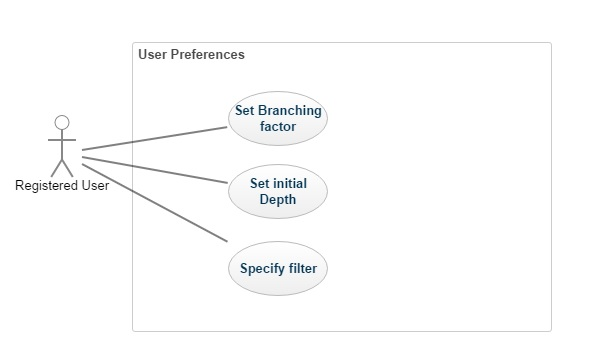
\includegraphics[width=\linewidth]{User Preferences.jpg}
		\caption{Use Case: User Preferences}
		\end{figure}
		\begin{figure}
			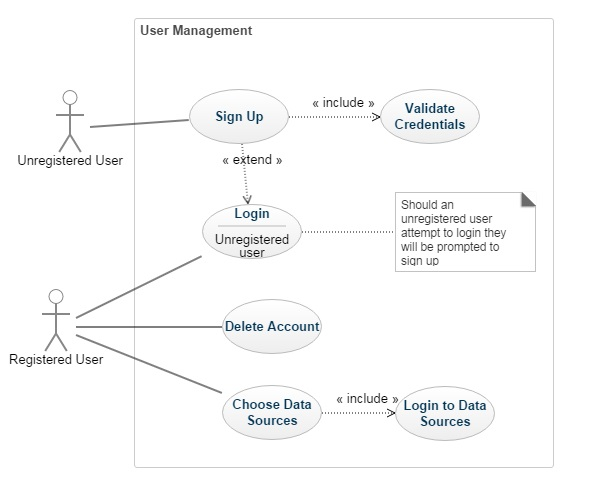
\includegraphics[width=\linewidth]{UserManagement.jpg}
			\caption{Use Case: User Management}
		\end{figure}
		\begin{figure}
			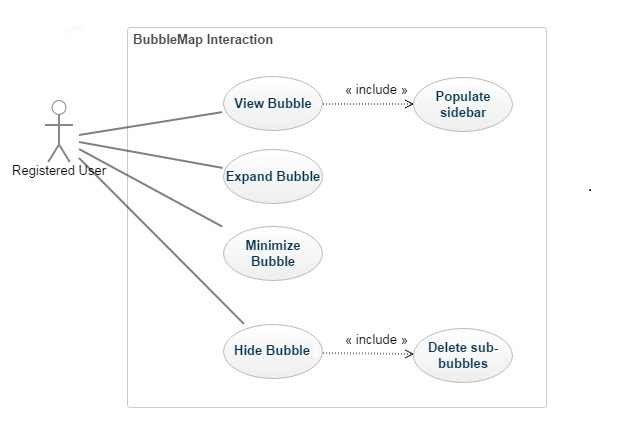
\includegraphics[width=\linewidth]{BubbleMap Interaction.jpg}
			\caption{Use Case: Bubble Map}
		\end{figure}
	
		\subsection{Required Functionality}
			Functionality that should be included in the system includes:
			\begin{itemize}
			\item A login/sign up system. 
			\item Adding various PIMs to your account.
			\item Interaction with PIMs directly from the mind map itself (commenting, emailing, etc).
			\item Expanding bubbles in order to find articles related to that bubble.
			\item Rapidly integrate new information into the system.
			\end{itemize}
	
	\section{Open Issues}
	
\end{document}
